\section{Annexes}
\subsection{Photos}
\begin{frame}
    \frametitle{Annexe 1}
    \begin{figure}
        \includegraphics[scale=0.05]{./figures/chau_02.jpg}
    \end{figure}
\end{frame}
\begin{frame}
    \frametitle{Annexe 2}
    \begin{figure}
        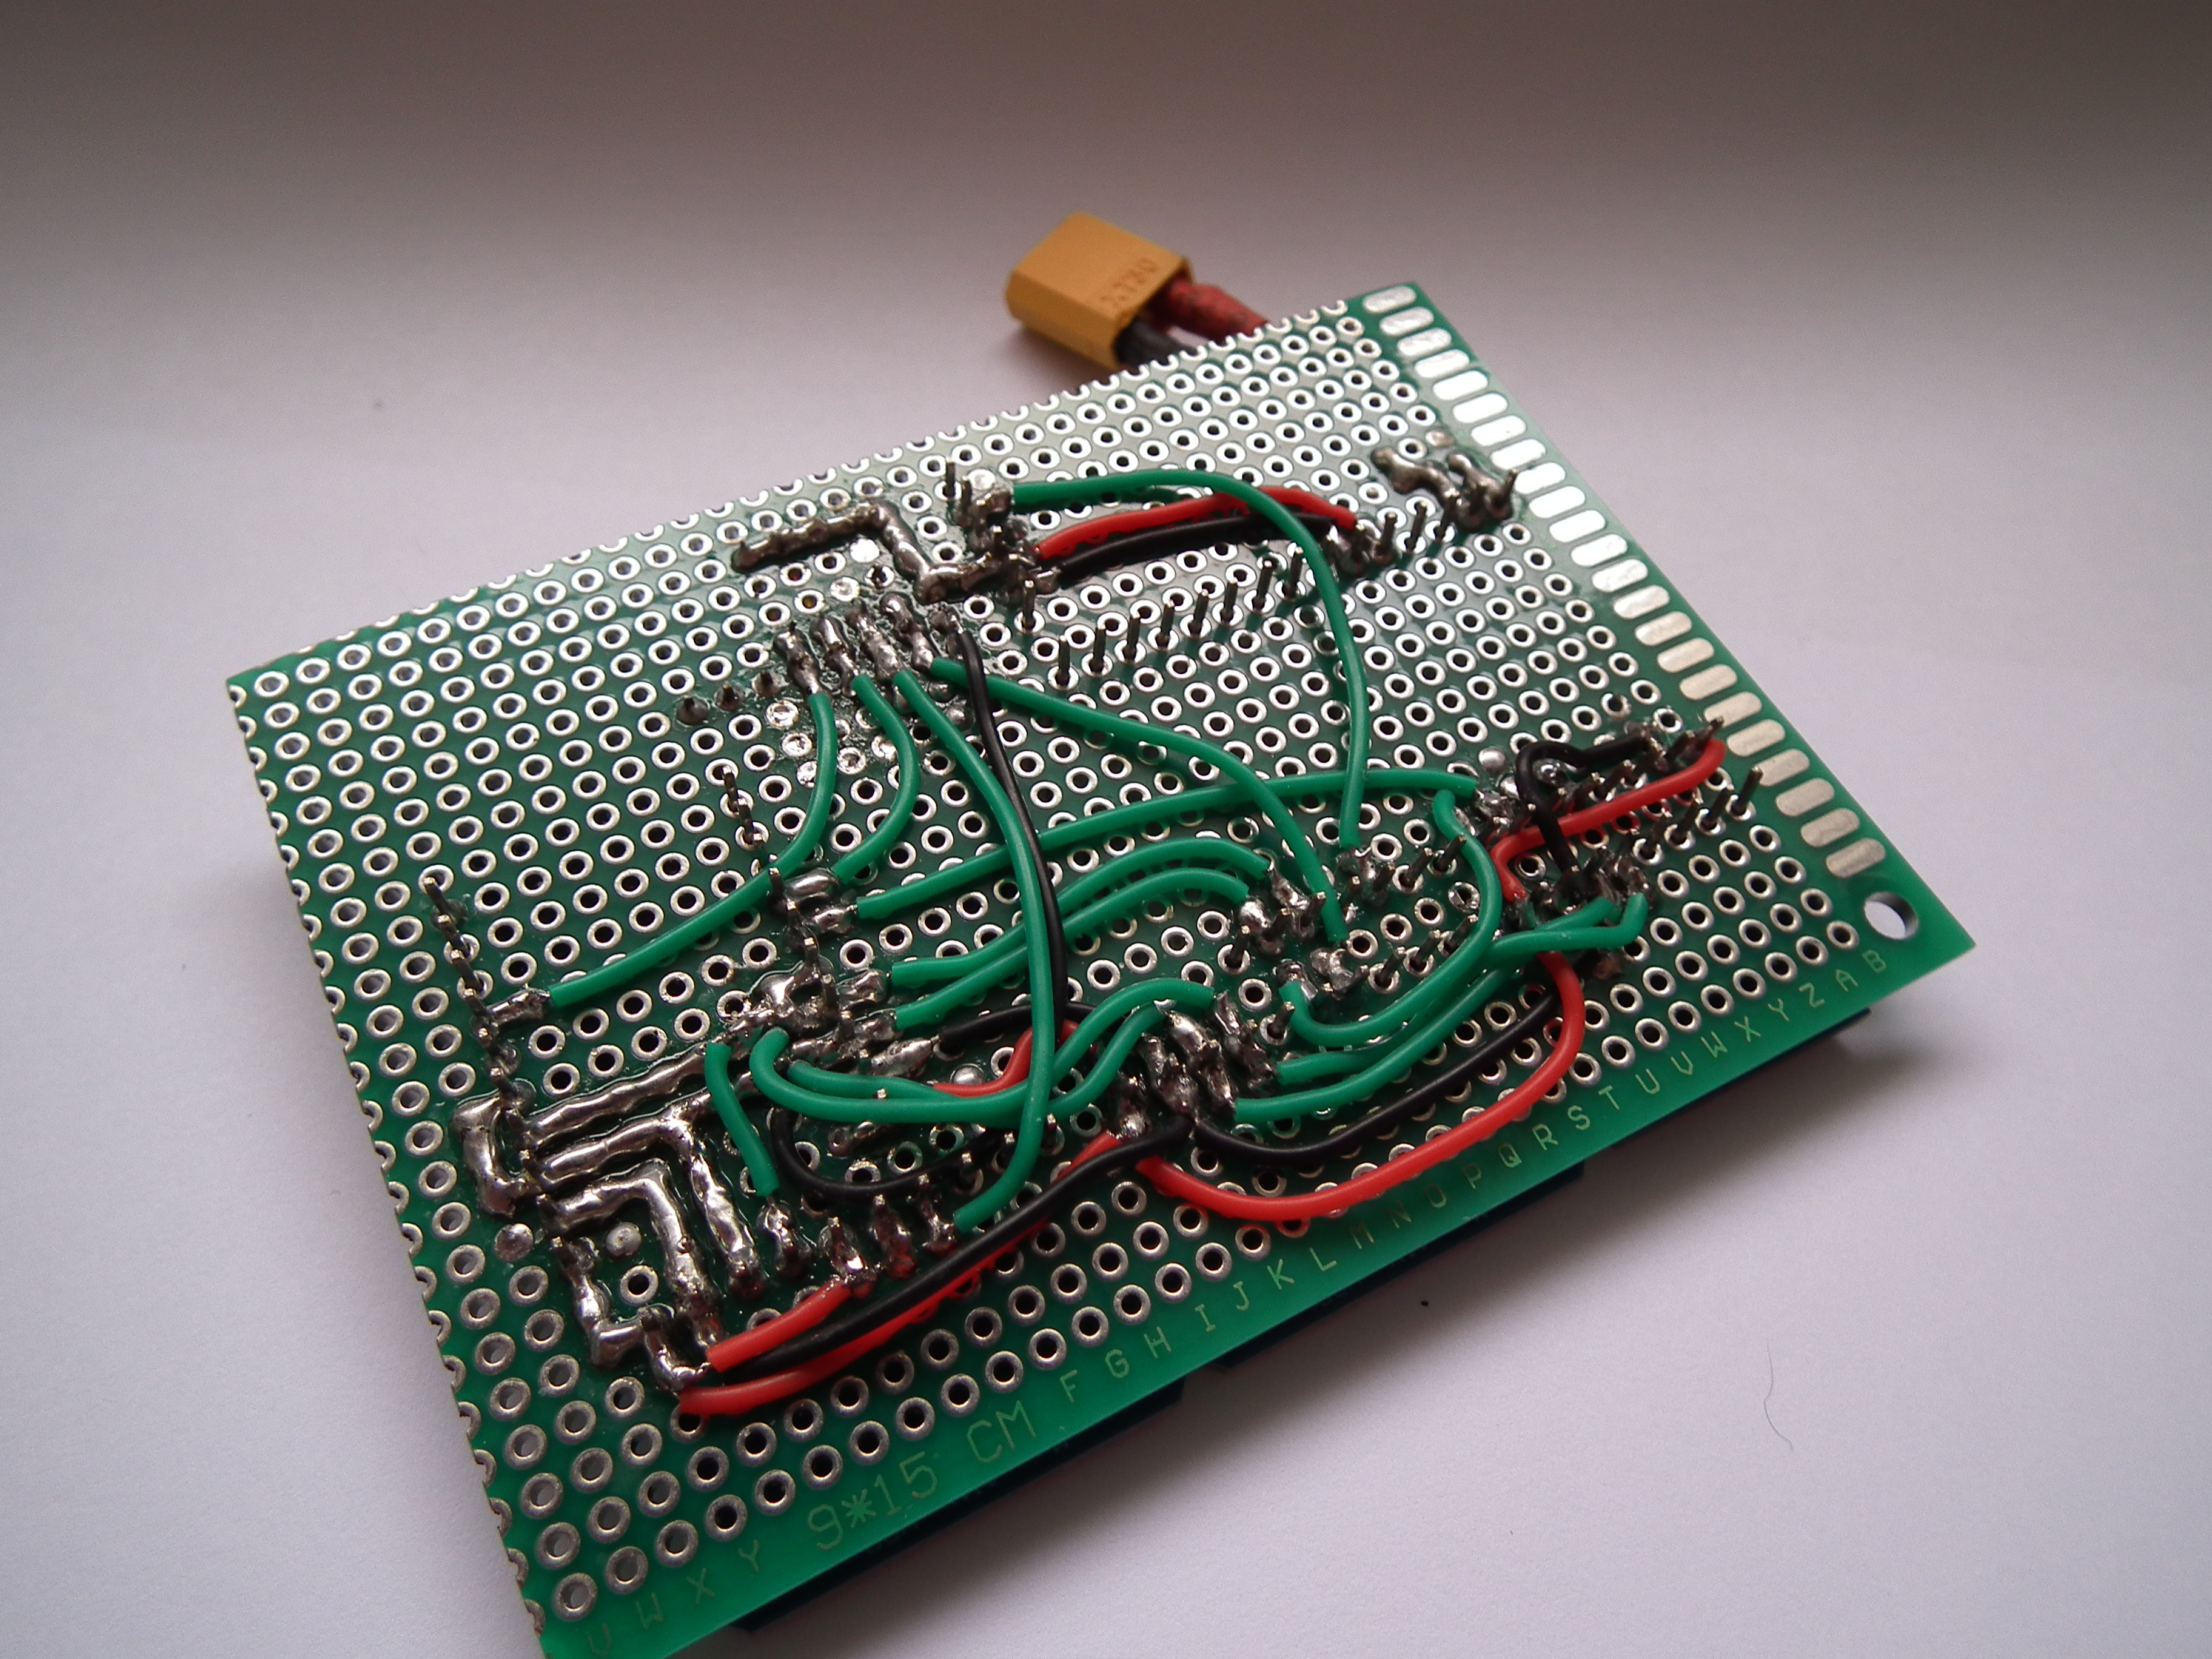
\includegraphics[scale=0.08]{./figures/carte_02.jpg}
    \end{figure}
\end{frame}
\begin{frame}
    \frametitle{Annexe 3}
    \begin{figure}
        \includegraphics[scale=0.1]{./figures/sem_03.jpg}
    \end{figure}
\end{frame}
\begin{frame}
    \frametitle{Annexe 4}
    \begin{figure}
        \includegraphics[scale=0.4]{./figures/rheo_03.png}
    \end{figure}
\end{frame}
\begin{frame}
    \frametitle{Annexe 5}
    \begin{figure}
        \includegraphics[scale=0.4]{./figures/rheo_04.png}
    \end{figure}
\end{frame}
\subsection{Codes}
\begin{frame}
    \frametitle{Annexe 6}
    \lstinputlisting[language=C++, basicstyle=\tiny, linerange={140-147,160-177}]{../Code/Tipe/include/math/fitting/gradient_desc.hpp}
\end{frame}
\begin{frame}
    \frametitle{Annexe 7}
    \lstinputlisting[language=C++, basicstyle=\tiny, linerange={179-208}]{../Code/Tipe/include/math/fitting/gradient_desc.hpp}
\end{frame}
\begin{frame}
    \frametitle{Annexe 8}
    \lstinputlisting[language=C++, basicstyle=\tiny, linerange={209-226}]{../Code/Tipe/include/math/fitting/gradient_desc.hpp}
\end{frame}